\chapter{Marco teórico}
\label{ch:marco-teorico}

\section{Inteligencia artificial}

La \gls{ia} se puede definir como el estudio y diseño de agentes inteligentes, es decir, de sistemas que perciben su entorno y toman decisiones o acciones que maximizan sus posibilidades de éxito. Este campo se basa en disciplinas como la informática, la lógica o la neurociencia, que contribuyen a la simulación de capacidades cognitivas humanas en máquinas.

Los agentes inteligentes, que son la base de este campo, se clasifican según la capacidad de reconocer y actuar en su entorno. Podemos encontrar desde agentes simples, que responden directamente a estímulos, hasta agentes basados en utilidad, que evalúan si los resultados de sus acciones son satisfactorios. Es fundamental la racionalidad, la habilidad de realizar elecciones óptimas que maximicen la posibilidad de alcanzar objetivos. Utilizando distintas herramientas de lógica, los agentes inteligentes pueden formular y modificar conocimientos, deduciendo nueva información.

El razonamiento lógico es también fundamental para el desarrollo de algoritmos evolutivos, donde las decisiones sobre selección, cruzamiento o reproducción se basan en decisiones lógicas. Subclase de los métodos de aprendizaje automático inspirados en los procesos biológicos de evolución, aplican estos principios para desarrollar soluciones a complejos problemas.

A medida que la tecnología evoluciona, también lo hace la capacidad de la IA para aprender y adaptarse, al igual que los algoritmos genéticos mejoran a lo largo de las generaciones. Su implementación es cada vez mayor en campos como el desarrollo de software o la robótica, donde las mejoras en la optimización y en la resolución de los problemas conducen a mejoras significativas en la eficiencia y la funcionalidad.


\section{Algoritmos genéticos}

Un algoritmo se puede definir como un procedimiento computacional bien definido que toma un valor, o un conjunto de valores, como entrada y produce un valor, o un conjunto de valores, como salida. Se trata de un conjunto de instrucciones que permiten realizar una actividad mediante sucesivos pasos.

Un algoritmo evolutivo es un tipo de algoritmo que proviene de la computación evolutiva. Esta rama de la IA emplea principios inspirados en la evolución biológica para la resolución de problemas. Teoría propuesta por Charles Darwin en 1859, expone que en la naturaleza, en un entorno dado que puede albergar un número limitado de individuos, la selección natural favorecería a aquellos que poseyeran características que les permitiesen adaptarse mejor al medio, teniendo una mayor posibilidad de sobrevivir y reproducirse. A lo largo del tiempo, las características ventajosas se propagan a través de las generaciones, mientras que aquellas menos favorables tienden a desaparecer. Por lo tanto, estas poblaciones irán evolucionado y adaptándose gradualmente al entorno.

En 1975 John Holland propone imitar los procesos biológicos naturales que rigen la selección natural usando ordenadores, lo que sería el principio de los \glspl{ag}. En un AG, las soluciones son modeladas como individuos o cromosomas, que generalmente se representan como cadenas de bits, aunque también se puede usar otro tipo de cadenas. Estas soluciones son evaluadas por una función de aptitud o fitness, y las más adecuadas son selecciondas para reproducirse mediante cruzamiento y mutación, procesos que mezclan y alteran aleatoriamente los cromosomas para generar diversidad. Los descendientes resultantes forman nuevas generaciones que vuelven a ser evaluadas, creando un ciclo que se repite hasta cumplir alguna condición de parada, como pudiera ser un número limitado de generaciones o que se alcance la solución deseada.

\begin{figure}[H]
    \centering
    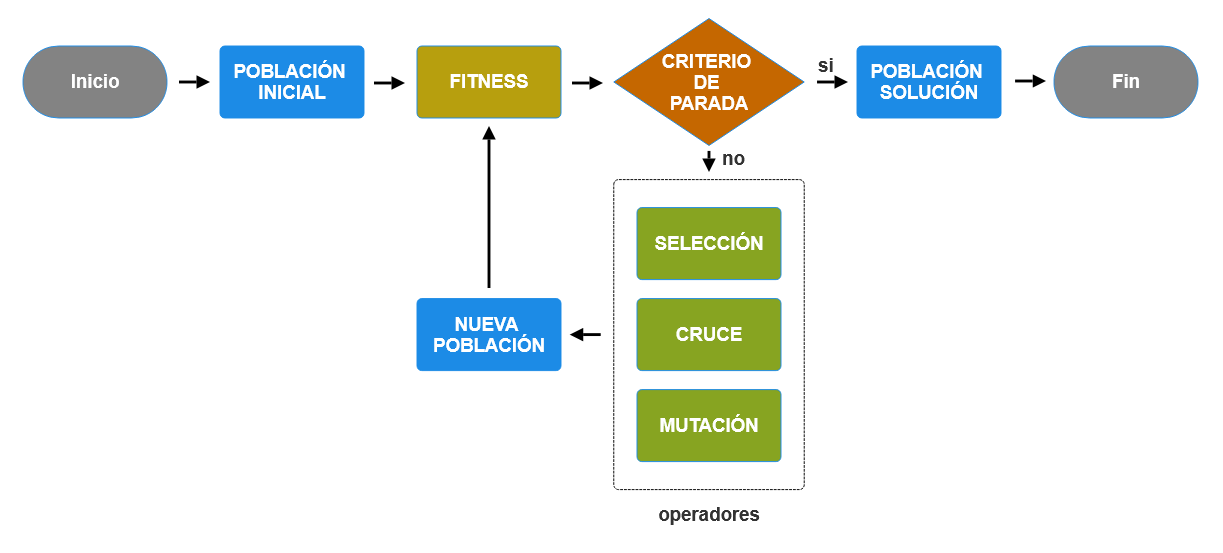
\includegraphics[width=1\textwidth]{figures/algoritmo-genetico.png}
    \caption{Algoritmo genético simple.}
    \label{fig:algoritmo-genetico}
  \end{figure}

Explicado el concepto general, se va a desglosar cada una de las fases de la figura \ref{fig:algoritmo-genetico}.

\subsection{Población}

Antes de explicar la generación de una población inicial, es necesario conocer algunos conceptos que son usados para representar y entender las soluciones. Son términos que son usados en la biología y en el campo de la genética. 

\begin{itemize}
    \item \textbf{Gen.} Es la unidad básica de información en un cromosoma. En una cadena de bits que representa una solución, cada bit puede considerarse un gen. En el caso que se trata en este PFG, el menú semanal, cada tipo de comida se podría considerar un gen. Por ejemplo, un gen sería bebida, plato principal o postre.
    \item \textbf{Alelo.} Es la forma específica o valor que puede tomar un gen. Siguiendo el ejemplo de bebida, posibles alelos serían agua, té o cerveza.
    \item \textbf{Cromosoma.} Es una colección de genes y representa una solución completa al problema de optimización. El cromosoma es la cadena de bits completa. En nuestro caso, la lista completa de alimentos seleccionados de un día determinado es el cromosoma. 
    \item \textbf{Fenotipo.} Es la manifestación real de la solución codificada. En el PFG sería cómo se preparan y sirven estos alimentos en la realidad.
\end{itemize}

La generación de una población inicial implica crear un conjunto de soluciones candidatas. Generalmente, los individuos son seleccionados aleatoriamente dentro de los límites definidos en cada problema, asegurando que todas las áreas del espacio de búsqueda puedan ser exploradas. También existen métodos alternativos de generación que aplican ciertas restricciones para formar soluciones iniciales más prometedoras. Tomando de ejemplo el menú semanal, el espacio de búsqueda comprendería la base de datos en la que aparecen todos los alimentos con sus respectivas calorias y macronutrientes. 

\begin{figure}[H]
  \centering
  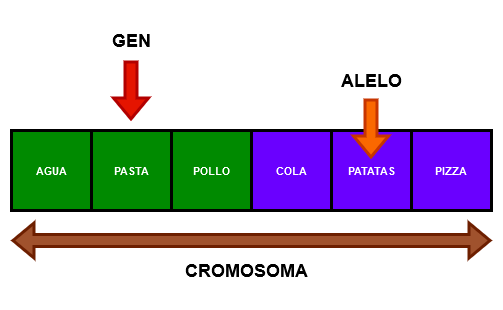
\includegraphics[width=0.625\textwidth]{figures/cromosoma.png}
  \caption{Estructura de un cromosoma.}
  \label{fig:cromosoma}
\end{figure}


\subsection{Evaluación}

Se mide lo bueno que es un individuo para nuestros propósitos (la calidad del individuo). Por lo tanto, lo más importante es definir una función de fitness correcta y representativa del problema a evaluar.

Según vayan pasando generaciones, la población inicial irá evolucionando hacia poblaciones candidatas que presentarán una mejor aptitud. Si la población ha alcanzado el objetivo, la condición de parada se activará, convirtiendo el conjunto de individuos candidatos en la población solución. En caso de no alcanzarlo, seguirá evolucionando hacia otra población candidata distinta.

\subsection{Operadores}

Son los procesos que se aplican a poblaciones de individuos para desarrollar generaciones futuras. Sirven para la exploración del espacio de soluciones y para la mejora de las poblaciones a través de las generaciones. Se busca que el conjunto de individuos presente una alta diversidad, ya que si es baja se corre el riego de caer en mínimos locales, lo que no permitiría explorar el espacio de soluciones ampliamente.


\subsubsection{Selección}

El primero de los operadores básicos. Elige un individuo para reproducirlo. Si bien se puede seleccionar de manera equiprobable, existen métodos basados en la aptitud del individuo. Estos son algunos:

\begin{itemize}
  \item \textbf{Método estándar (rueda de la fortuna).} Asigna a cada individuo una probabilidad proporcional a su fitness, por lo que los más aptos tienen mayor probabilidad de reproducirse. Existe un derivado de este método en el que se normalizan las probabilidades, lo que favorece aún más a los adaptados.
  \item \textbf{Método del rango.} Se ordenan los individuos según su aptitud, y la probabilidad de selección se asigna según este ránking.
  \item \textbf{Selección por torneo.} Se escoge aleatoriamente un subconjunto de individuos de la población, y el mejor de este es elegido.
\end{itemize}

La selección puede incorporar un mecanismo de elitismo, que escoge los mejores individuos de una generación para que se mantengan en la siguiente. Esto ayuda a que la calidad del mejor individuo de una generación sea siempre igual o superior a su equivalente de la generación anterior, consiguiendo una progresión constante hacia la solución óptima, es decir, una mayor convergencia.

También se debe buscar un equilibrio con la diversidad. Si no se explora el espacio de búsqueda en amplitud, se podría caer en mínimos locales si la población es muy parecida entre sí, lo que no permitiría encontrar buenas soluciones.


\subsubsection{Cruce}

Se combina el material genético de dos individuos, padres, para producir descendencia, hijos. Es decir, se utiliza para intercambiar características de dos soluciones parentales con el objetivo de generar nuevas soluciones. Se aplica con probabilidad \(P_c\) . Al promover la mezcla de genes, ayuda a aumentar la diversidad y la convergencia, debido a la generación de nuevos descendientes con características deseables. Para problemas donde las soluciones están representadas como cadena de bits o enteros, se usan distintos métodos:

\begin{itemize}
  \item \textbf{Cruce de un punto.} Se selecciona aleatoriamente una posición en el cromosoma. Todo lo que está antes de este punto se intercambia con todo lo que está después en la otra cadena, y viceversa, para producir dos descendientes.
  \item \textbf{Cruce de dos puntos.} Similar al cruce de un punto, pero se seleccionan dos puntos de corte. Las cadenas de genes entre estos dos puntos se intercambian entre los dos padres.
  \item \textbf{Cruce uniforme.} Cada gen tiene una probabilidad igual de ser elegido de uno de los dos padres.
\end{itemize}

\subsubsection{Mutación}

Último de los operadores básicos. Se recorre toda la cadena, mutando cada gen con probabilidad \(P_m\) , es decir, eligiendo un nuevo valor mediante una elección equiprobable sobre el alfabeto. La mutación aumenta la diversidad y ayuda a no caer en mínimos locales. Algunos de los métodos usados son:

\begin{itemize}
  \item \textbf{Mutación uniforme.} Cada gen puede cambiar a otro valor con probabilidad \(P_m\).
  \item \textbf{Mutación por intercambio.} Dos genes aleatorios en el cromosoma son seleccionados y sus posiciones se intercambian. 
\end{itemize}

\begin{figure}[H]
  \centering
  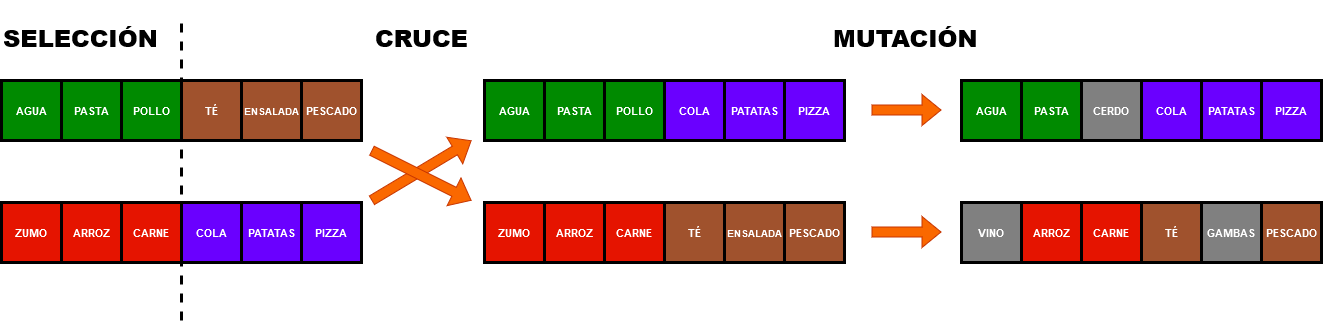
\includegraphics[width=1\textwidth]{figures/operadores.png}
  \caption{Operadores.}
  \label{fig:operadores}
\end{figure}